\documentclass{gescons}

\genre {Resumo do Biênio}
\author{Amanda Vieira}
\title{Editares no XXXVI Congraçamento das ICs: Plaquinhas, sorrisos e escrita}

\begin{document}
    \makeentrevistatitle
    %\maketitle

    %\fullwidthimage{fields}{b}

    %\coverart{back/editorial}
    \coverart{../fundo-generico.png}
    
%    \begin{multicols}{2}

%\begin{center}
%    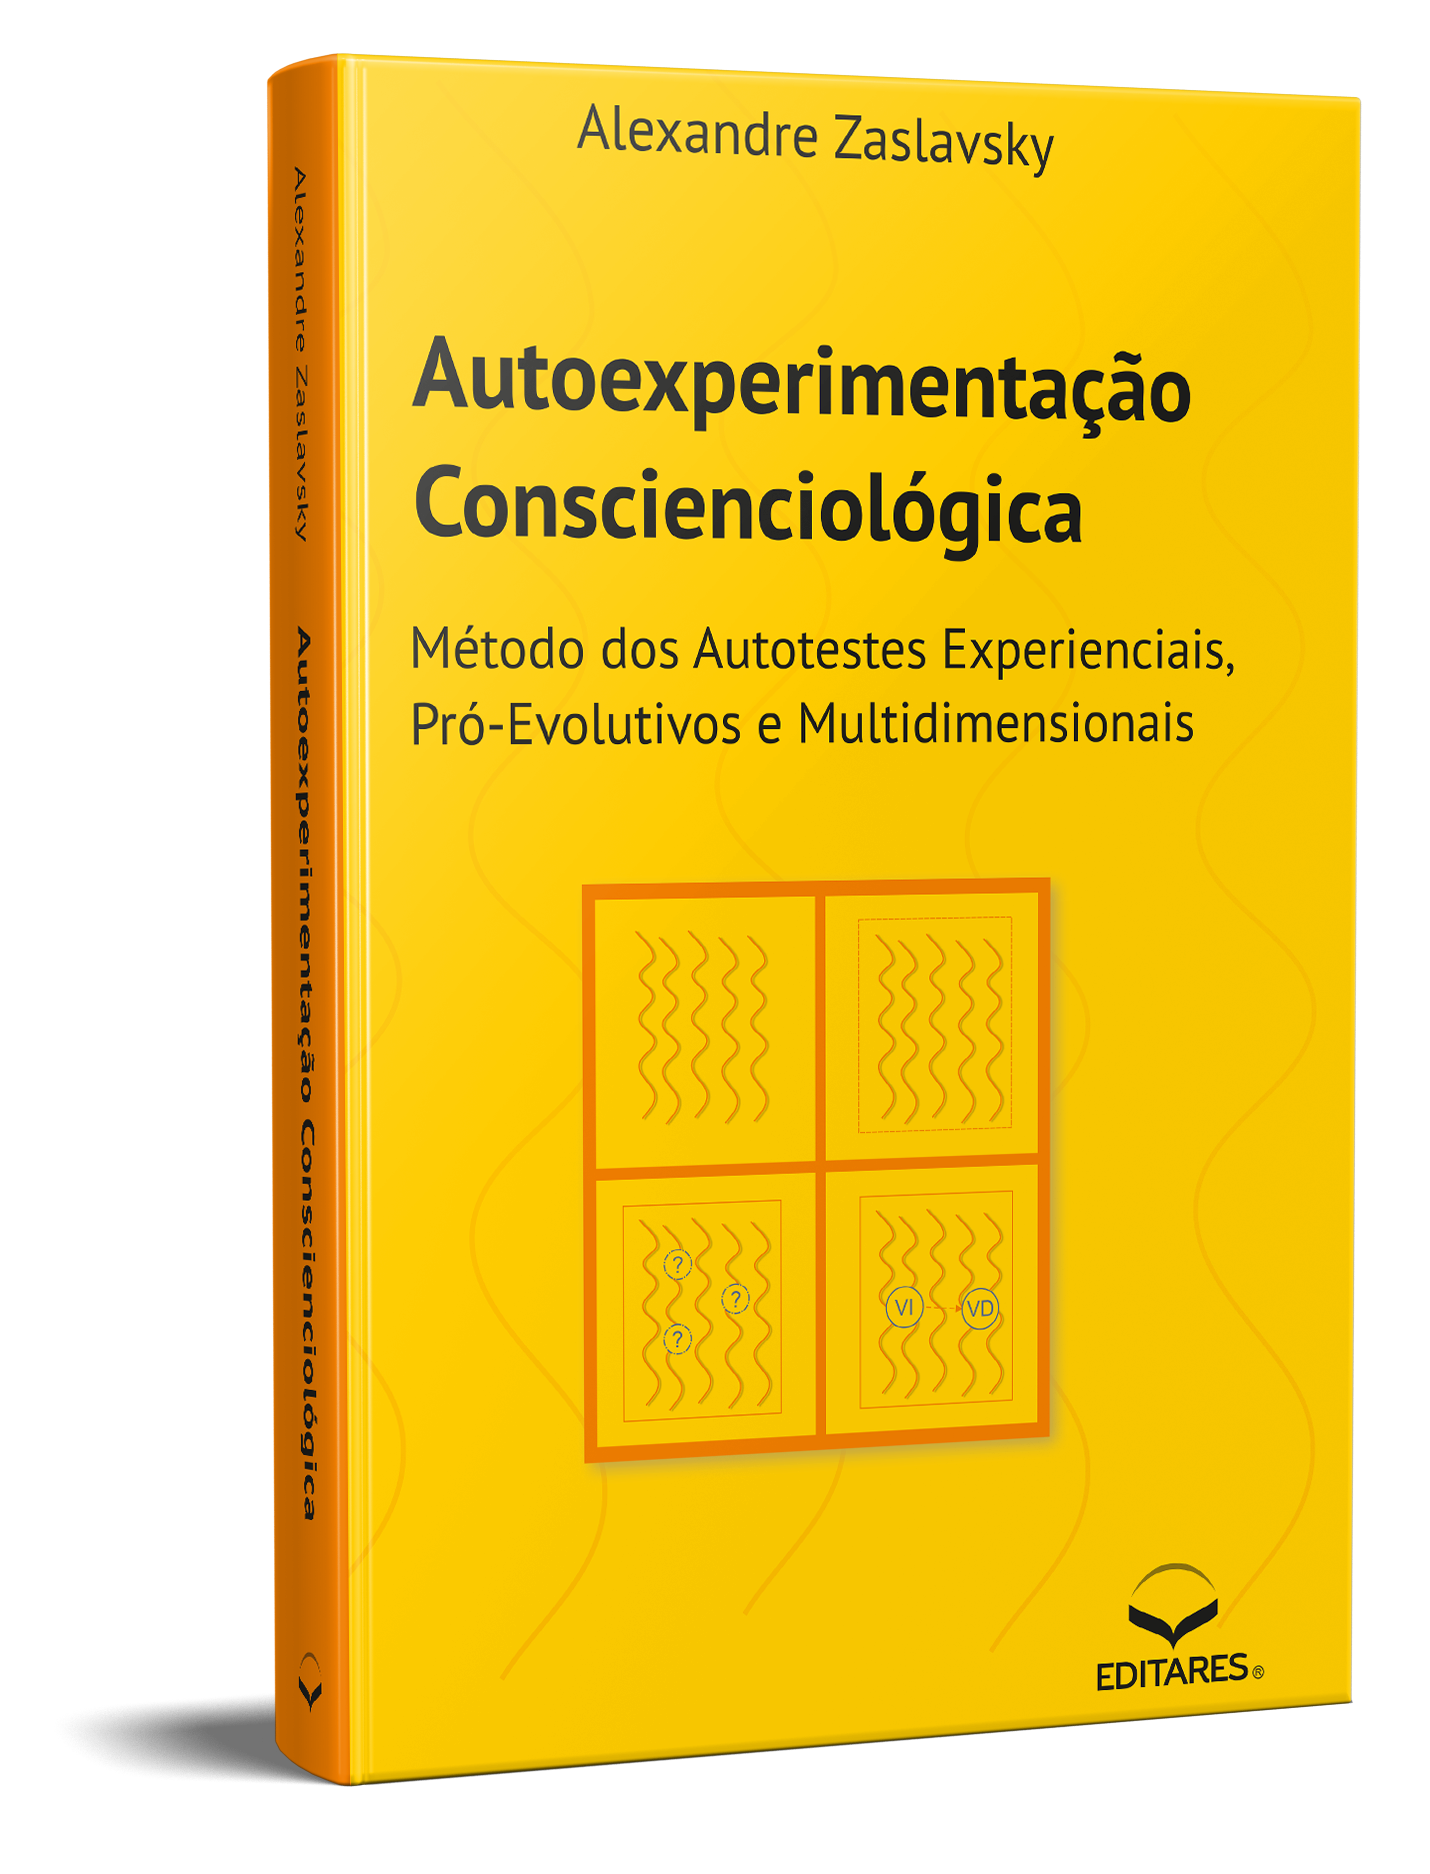
\includegraphics[width=4cm]{articles/entrevista/mockups/Alexandre-Zas.png}
%\end{center}





No dia 8 de dezembro de 2024, durante o tradicional \textbf{Congraçamento das ICs} -- evento anual de celebração do voluntariado conscienciológico --, a Editares marcou presença com uma ação voltada aos \textbf{autores e futuros autores}.

Com placas instigativas e frases de compromisso com a escrita, os voluntários foram convidados a tirar fotos simbolizando o engajamento na tarefa autoral. A atividade trouxe um clima de \textbf{descontração e leveza}, ao mesmo tempo em que reforçou a importância do autoposicionamento proexológico perante a escrita conscienciológica.

\textbf{Confira as fotos!}

  \begin{minipage}[b]{0.32\textwidth}
    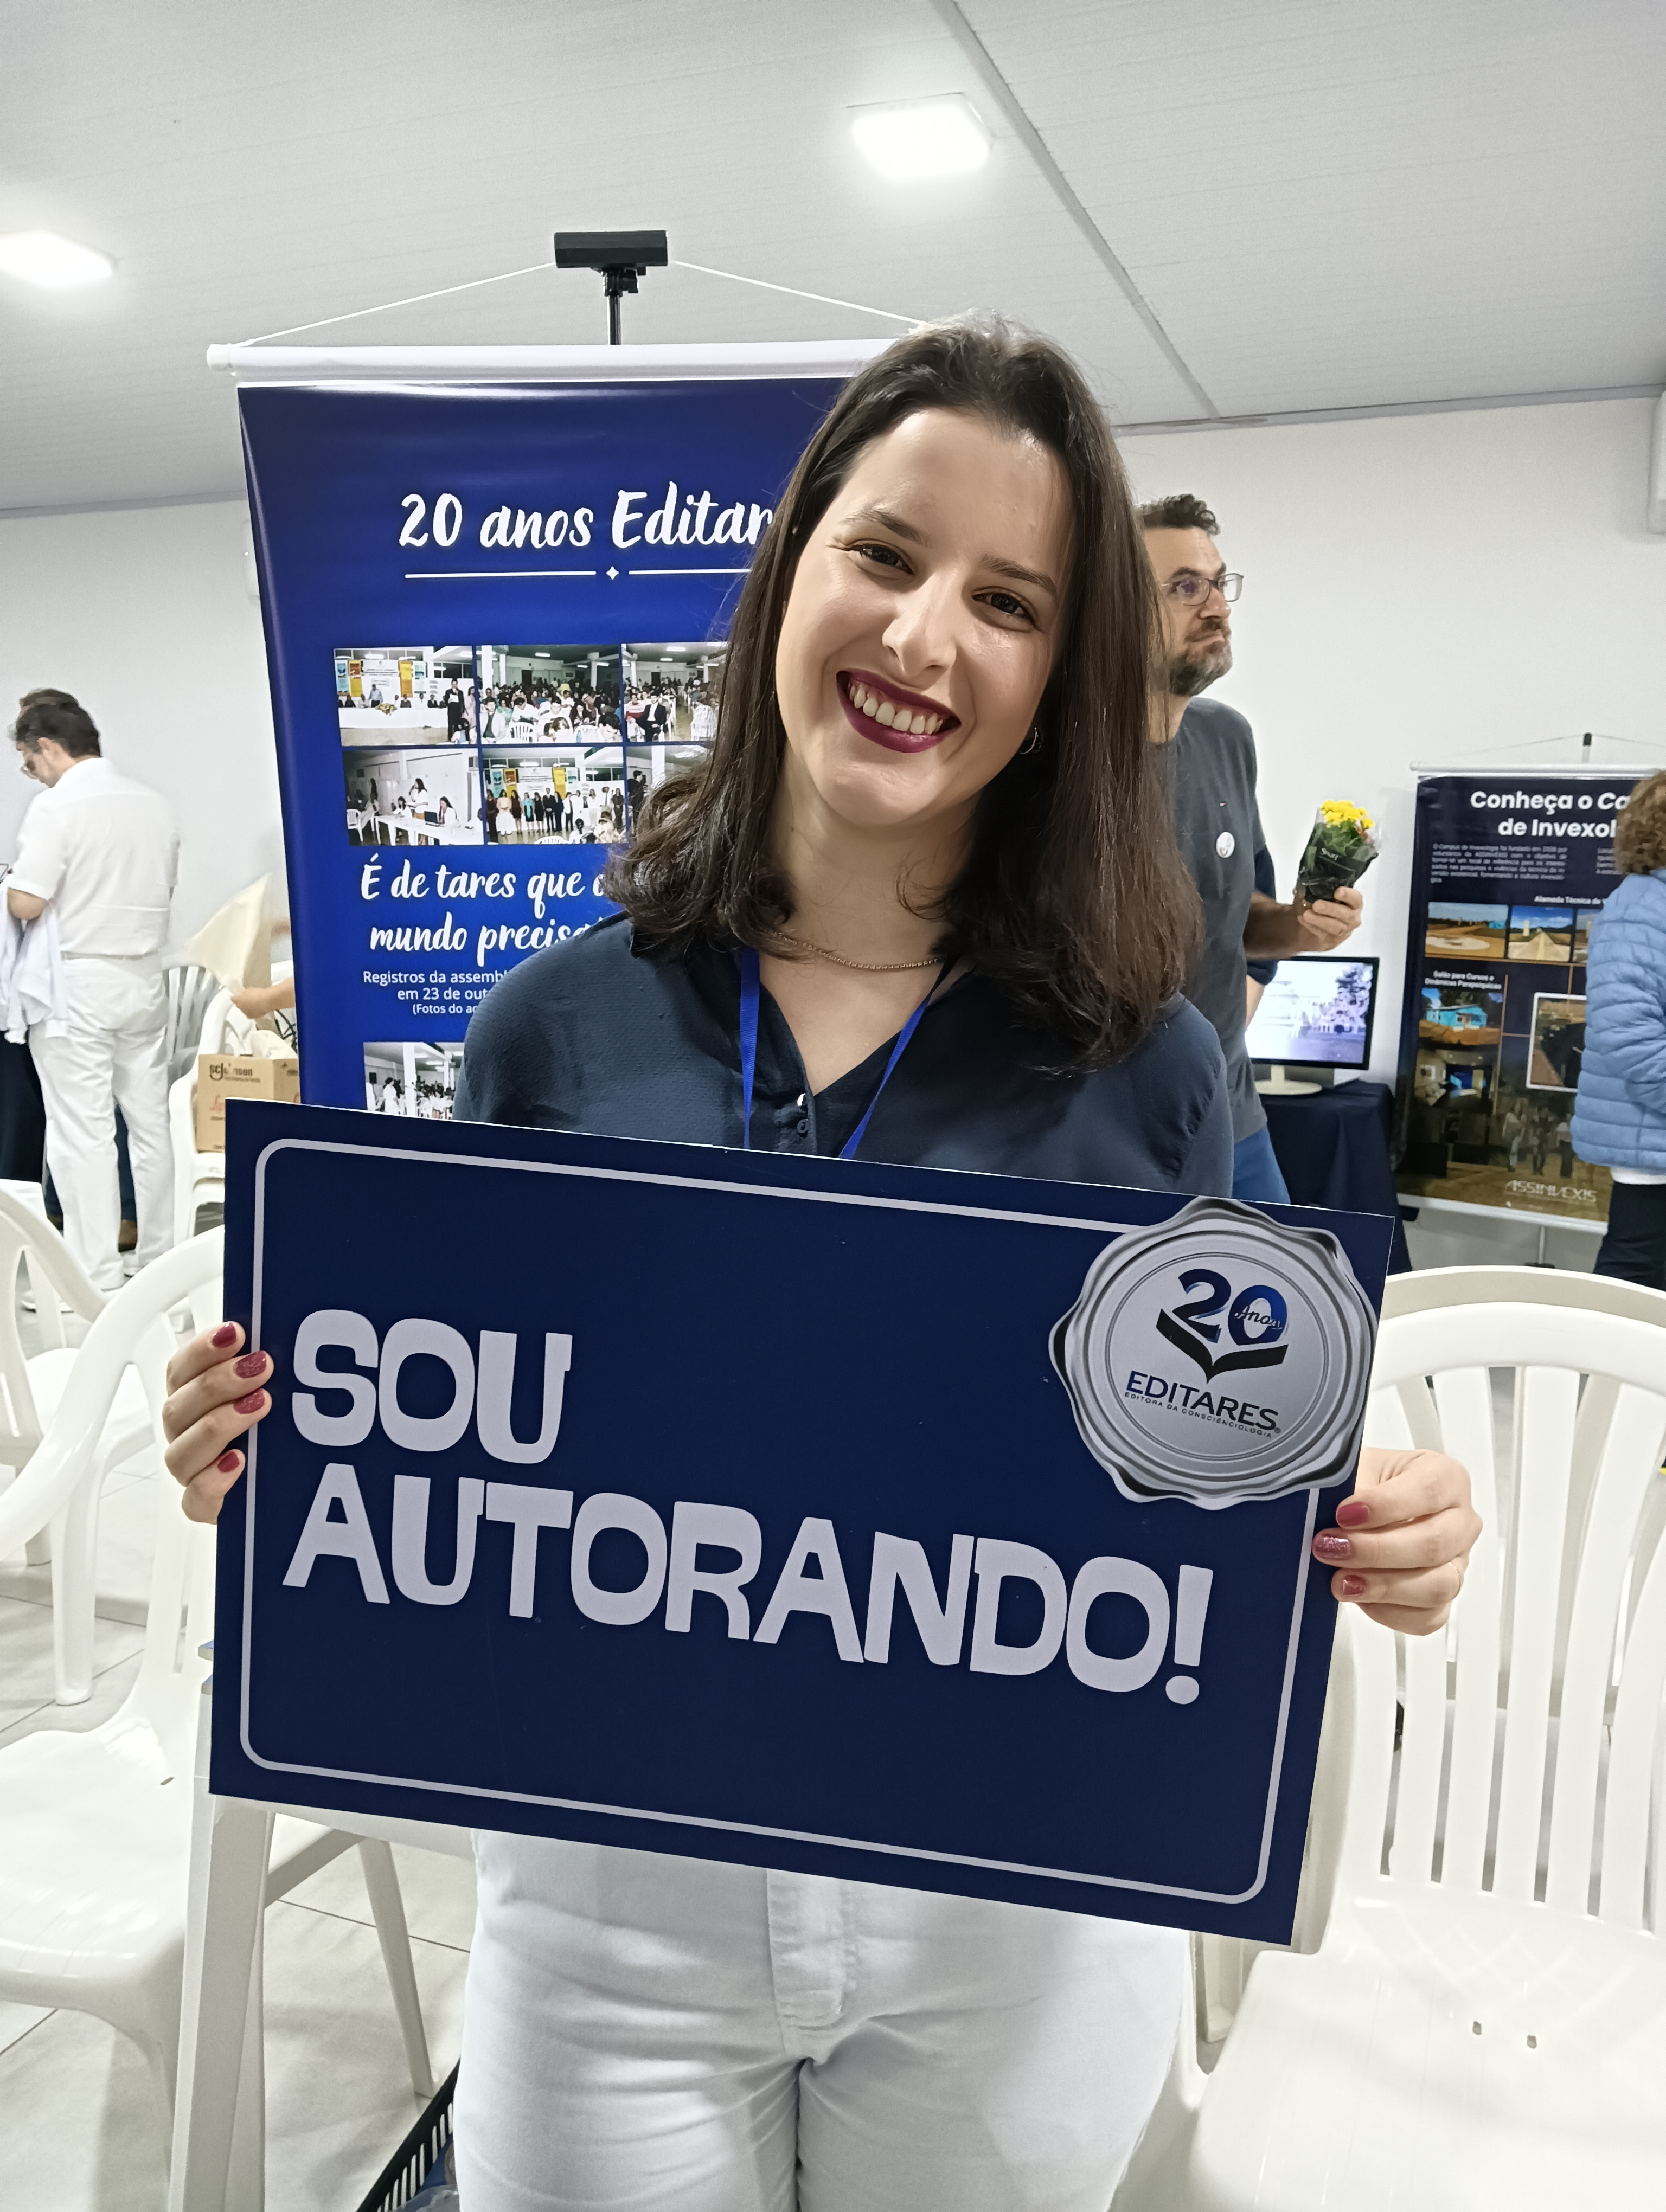
\includegraphics[width=\linewidth]{articles/resumo/fotos/materia2/IMG20241208144202.jpg}
  \end{minipage}\hfill
  \begin{minipage}[b]{0.32\textwidth}
    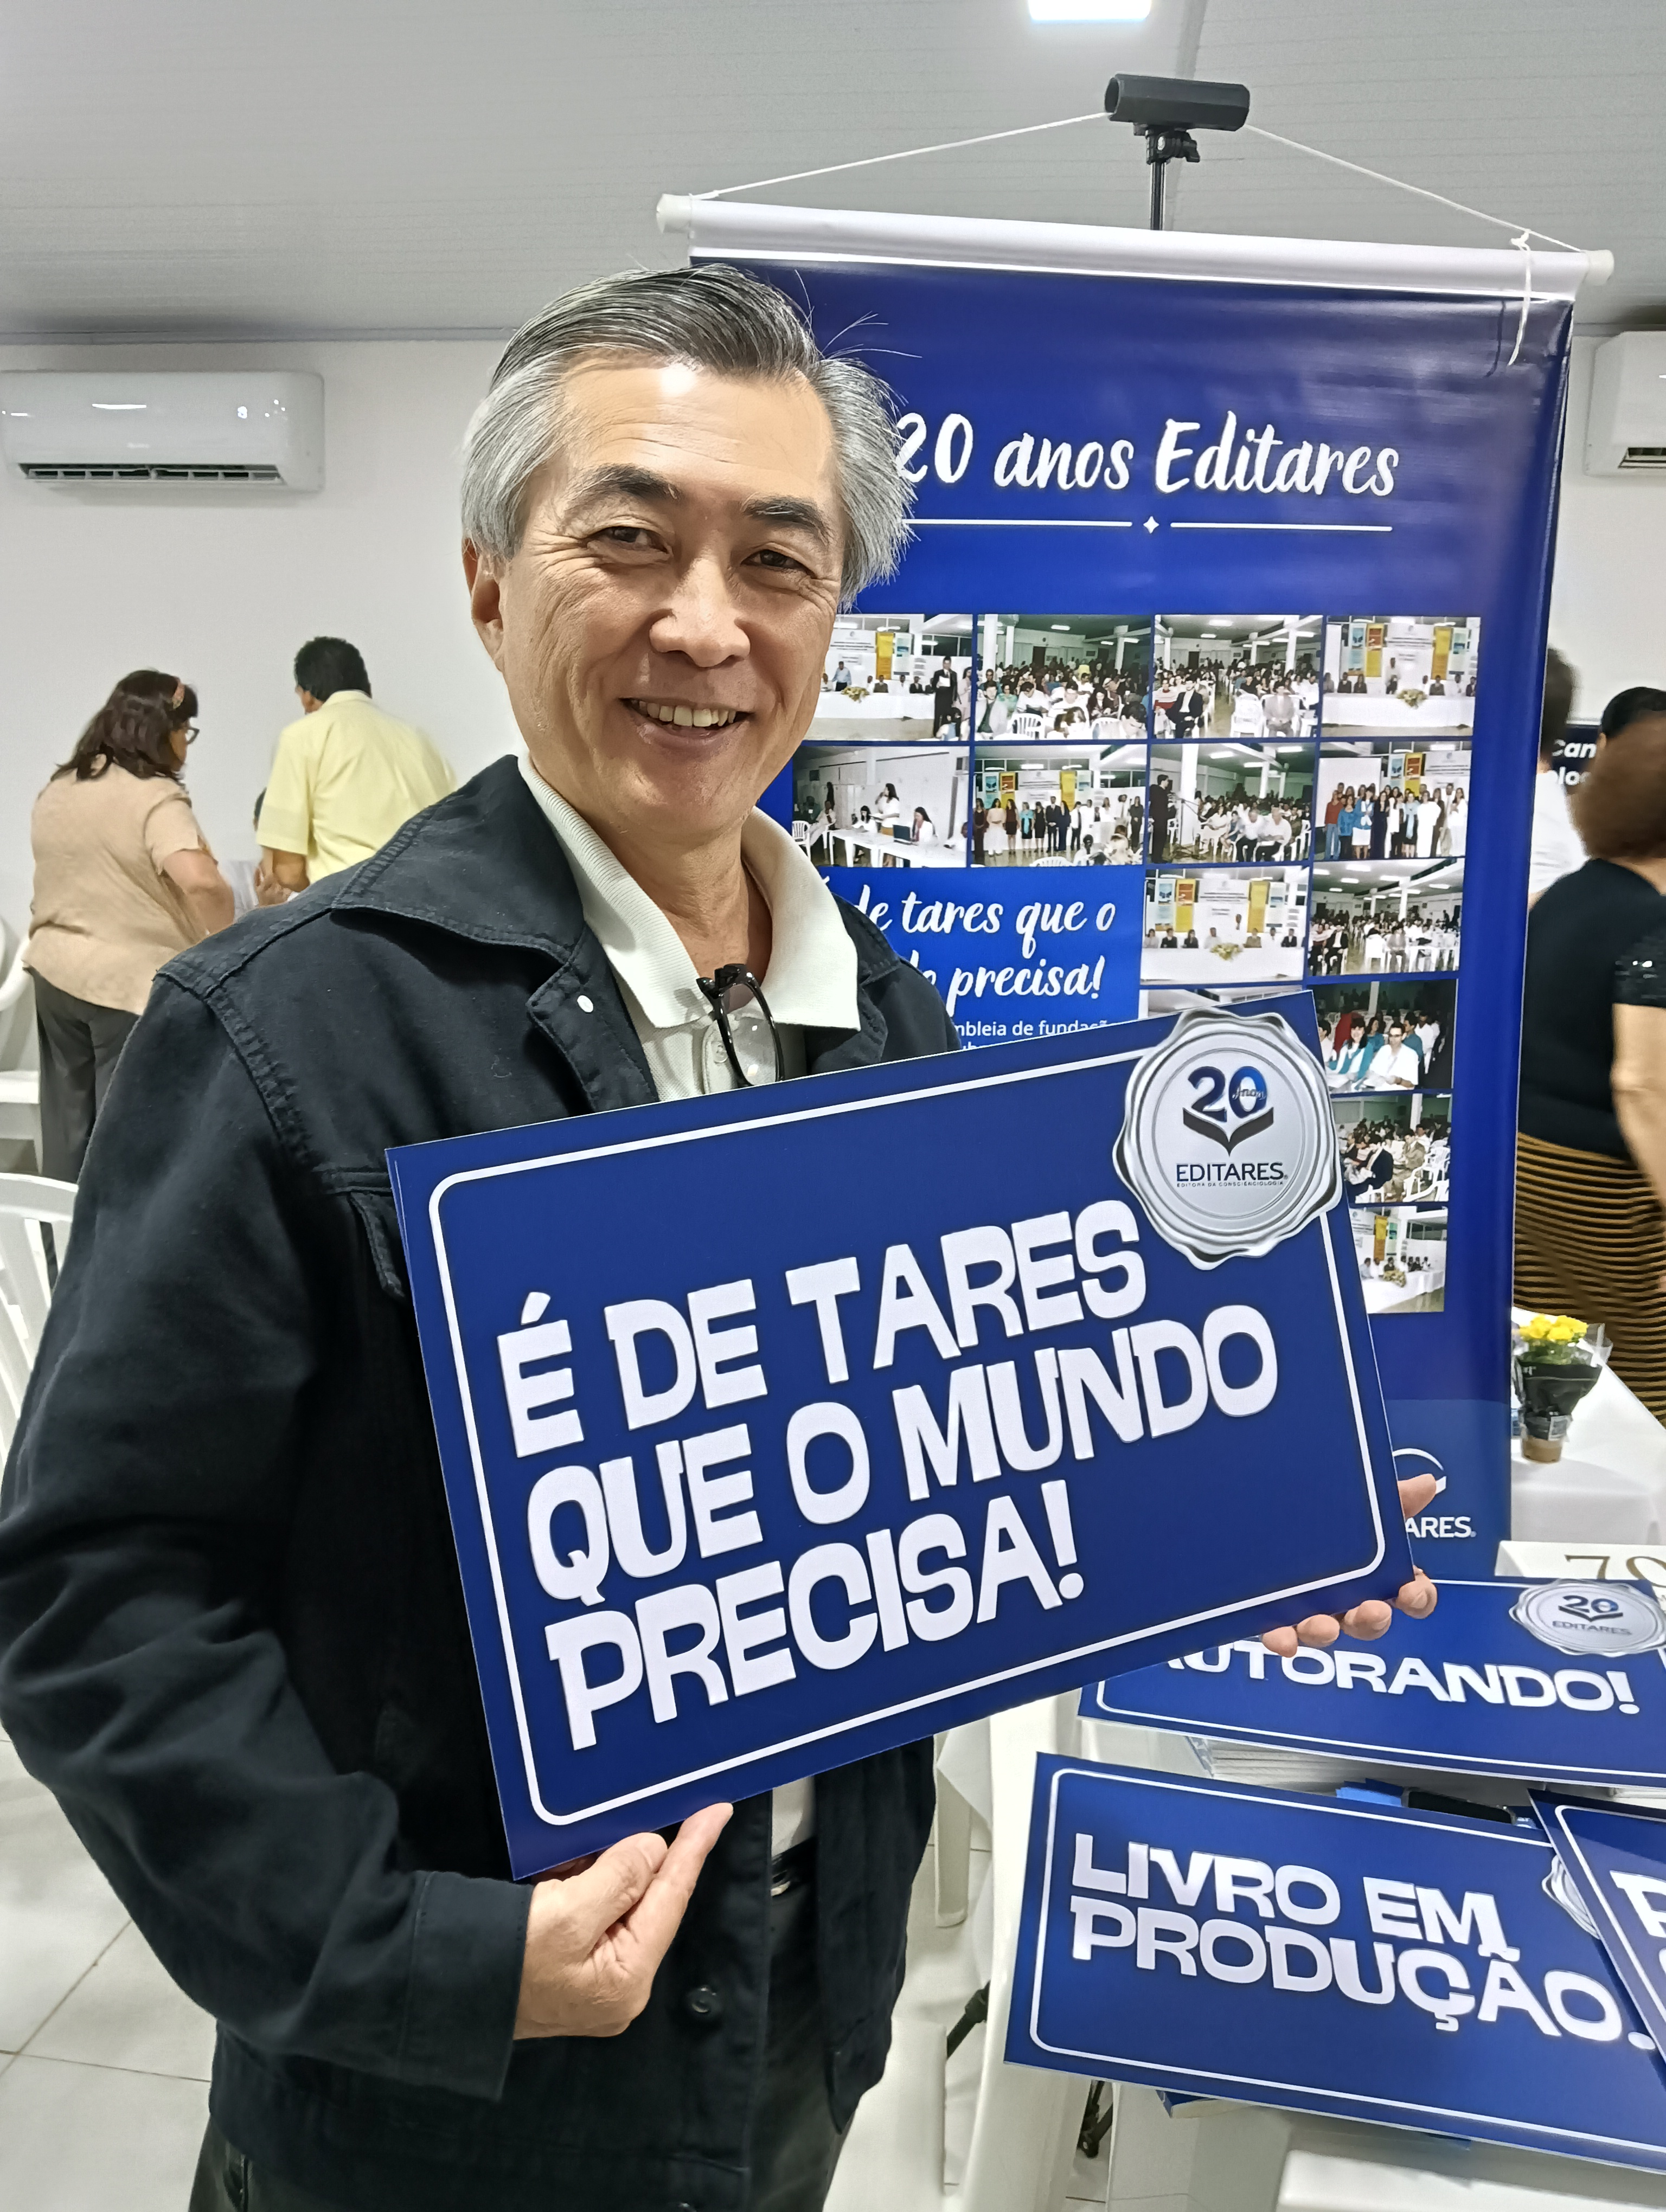
\includegraphics[width=\linewidth]{articles/resumo/fotos/materia2/IMG20241208145756.jpg}
  \end{minipage}\hfill
  \begin{minipage}[b]{0.32\textwidth}
    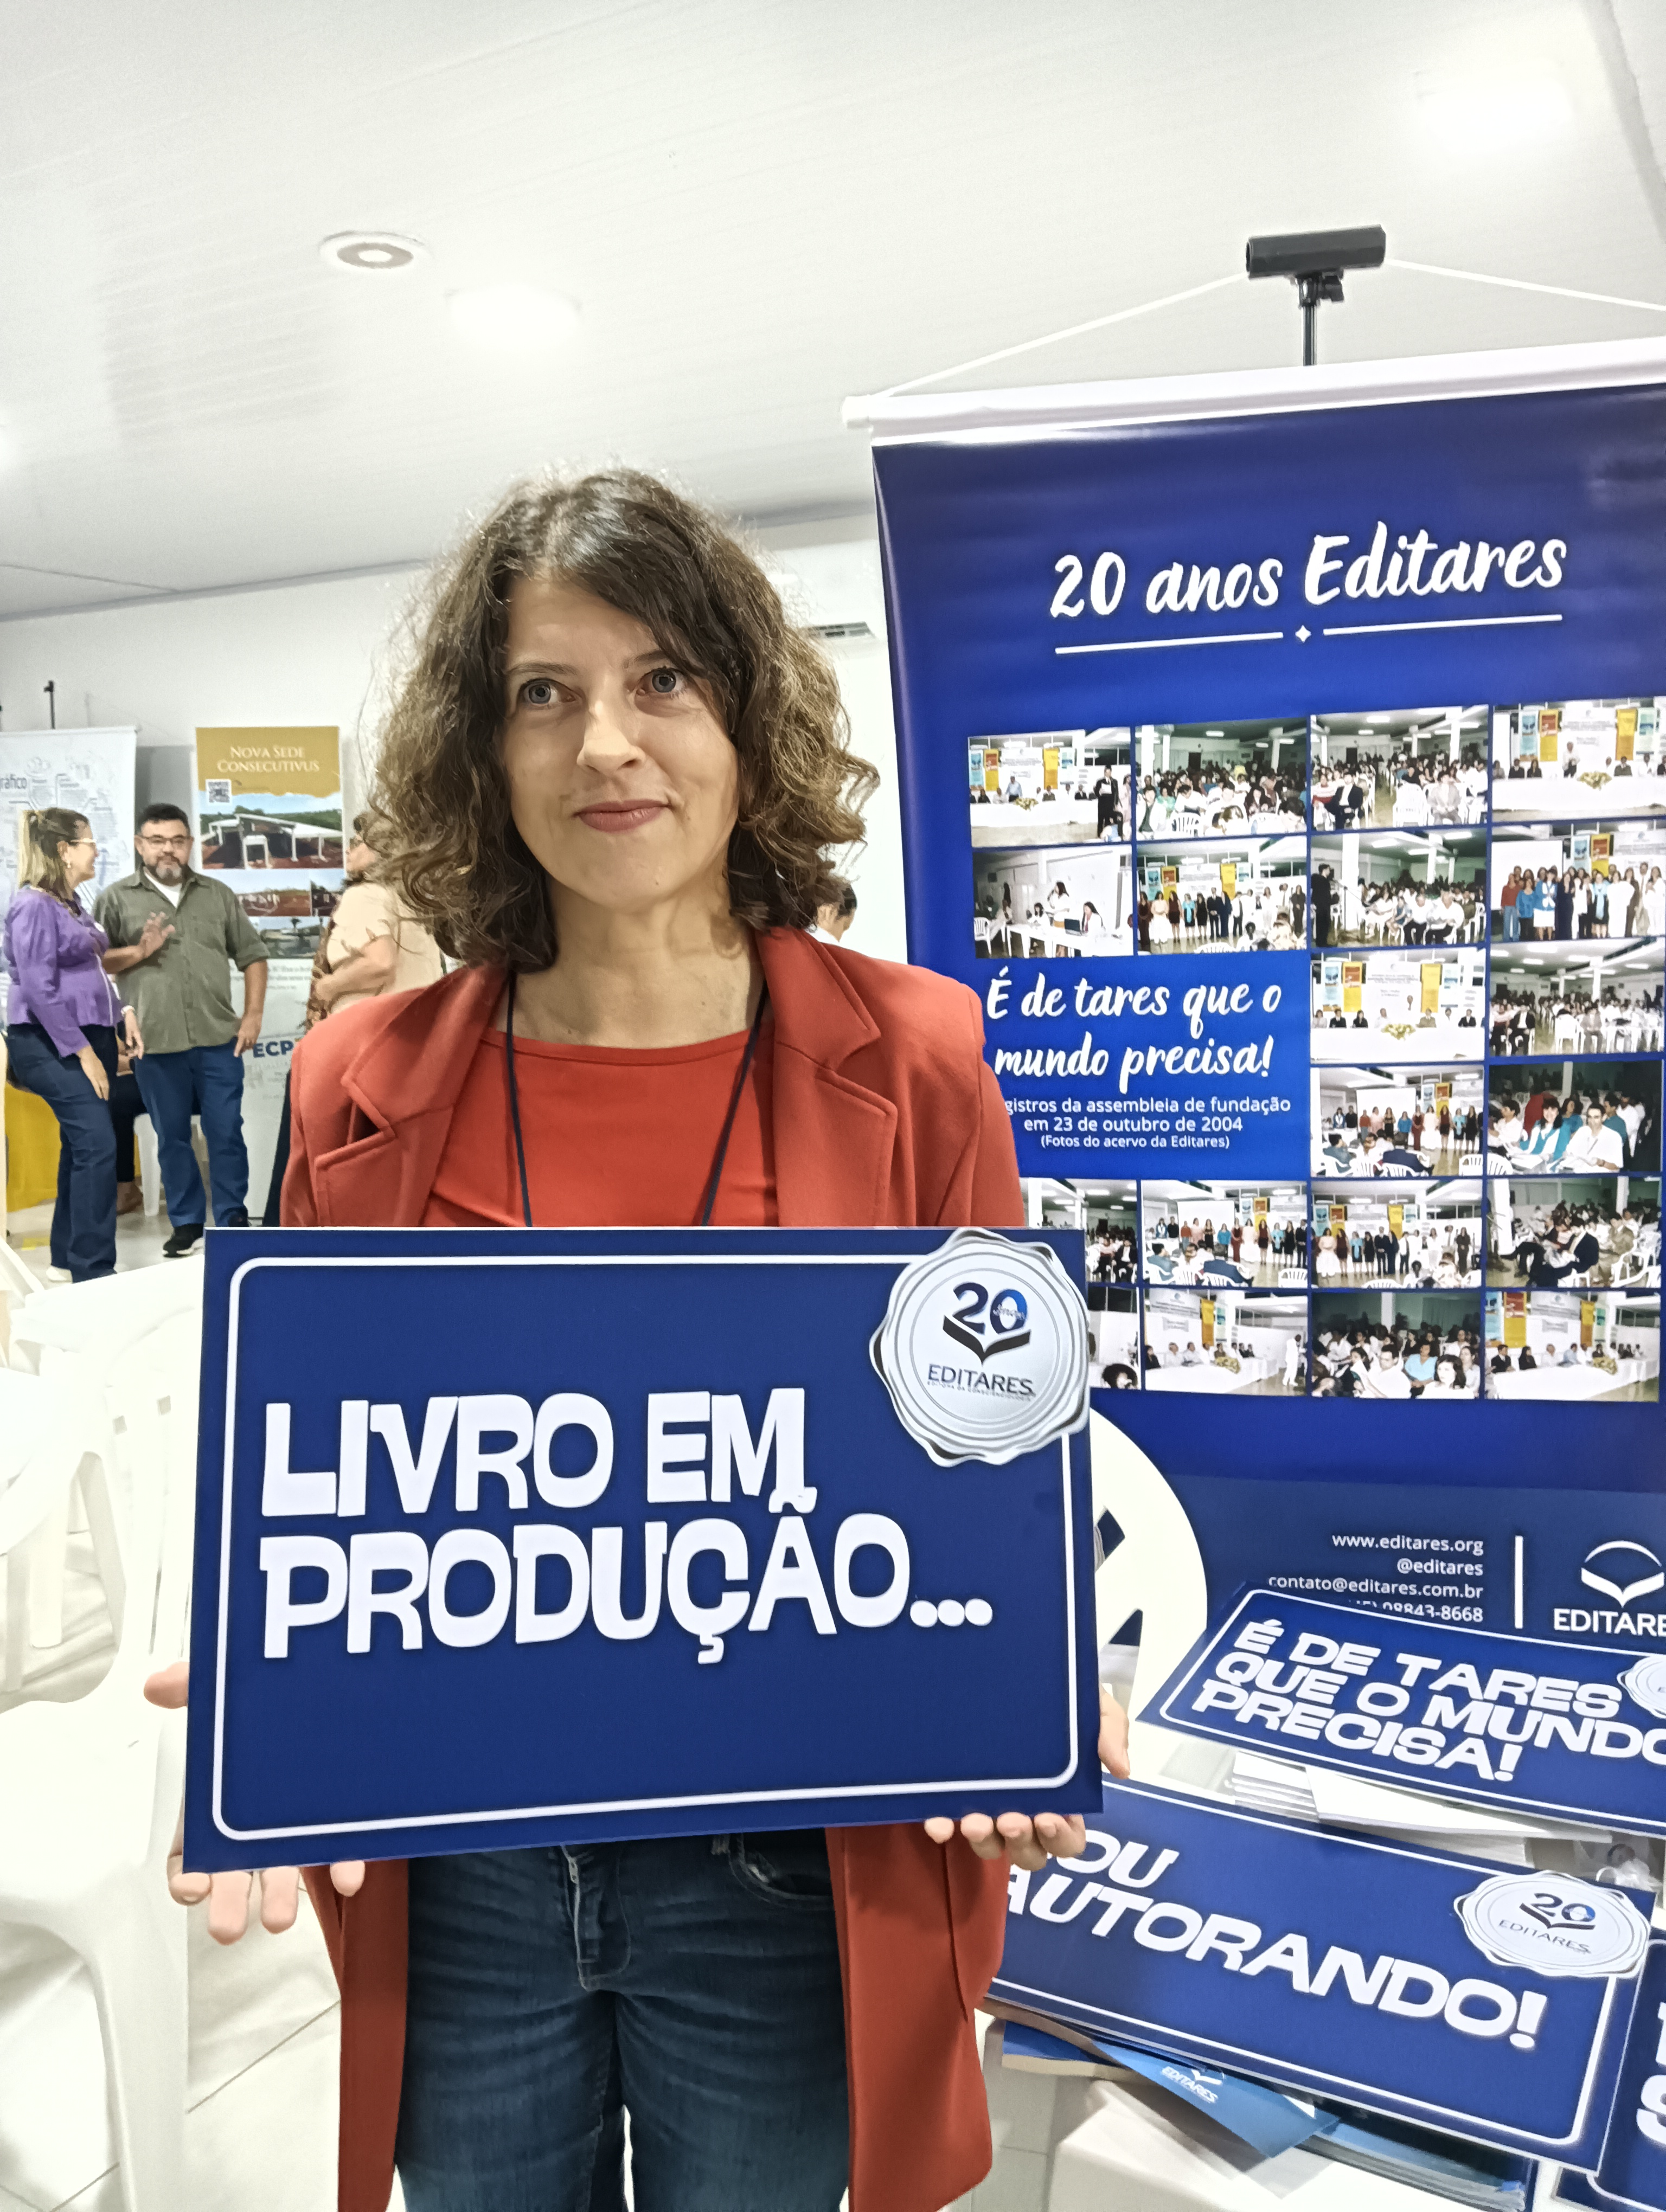
\includegraphics[width=\linewidth]{articles/resumo/fotos/materia2/IMG20241208144514.jpg}
  \end{minipage}
  
  \centering
  \begin{minipage}[b]{0.32\textwidth}
    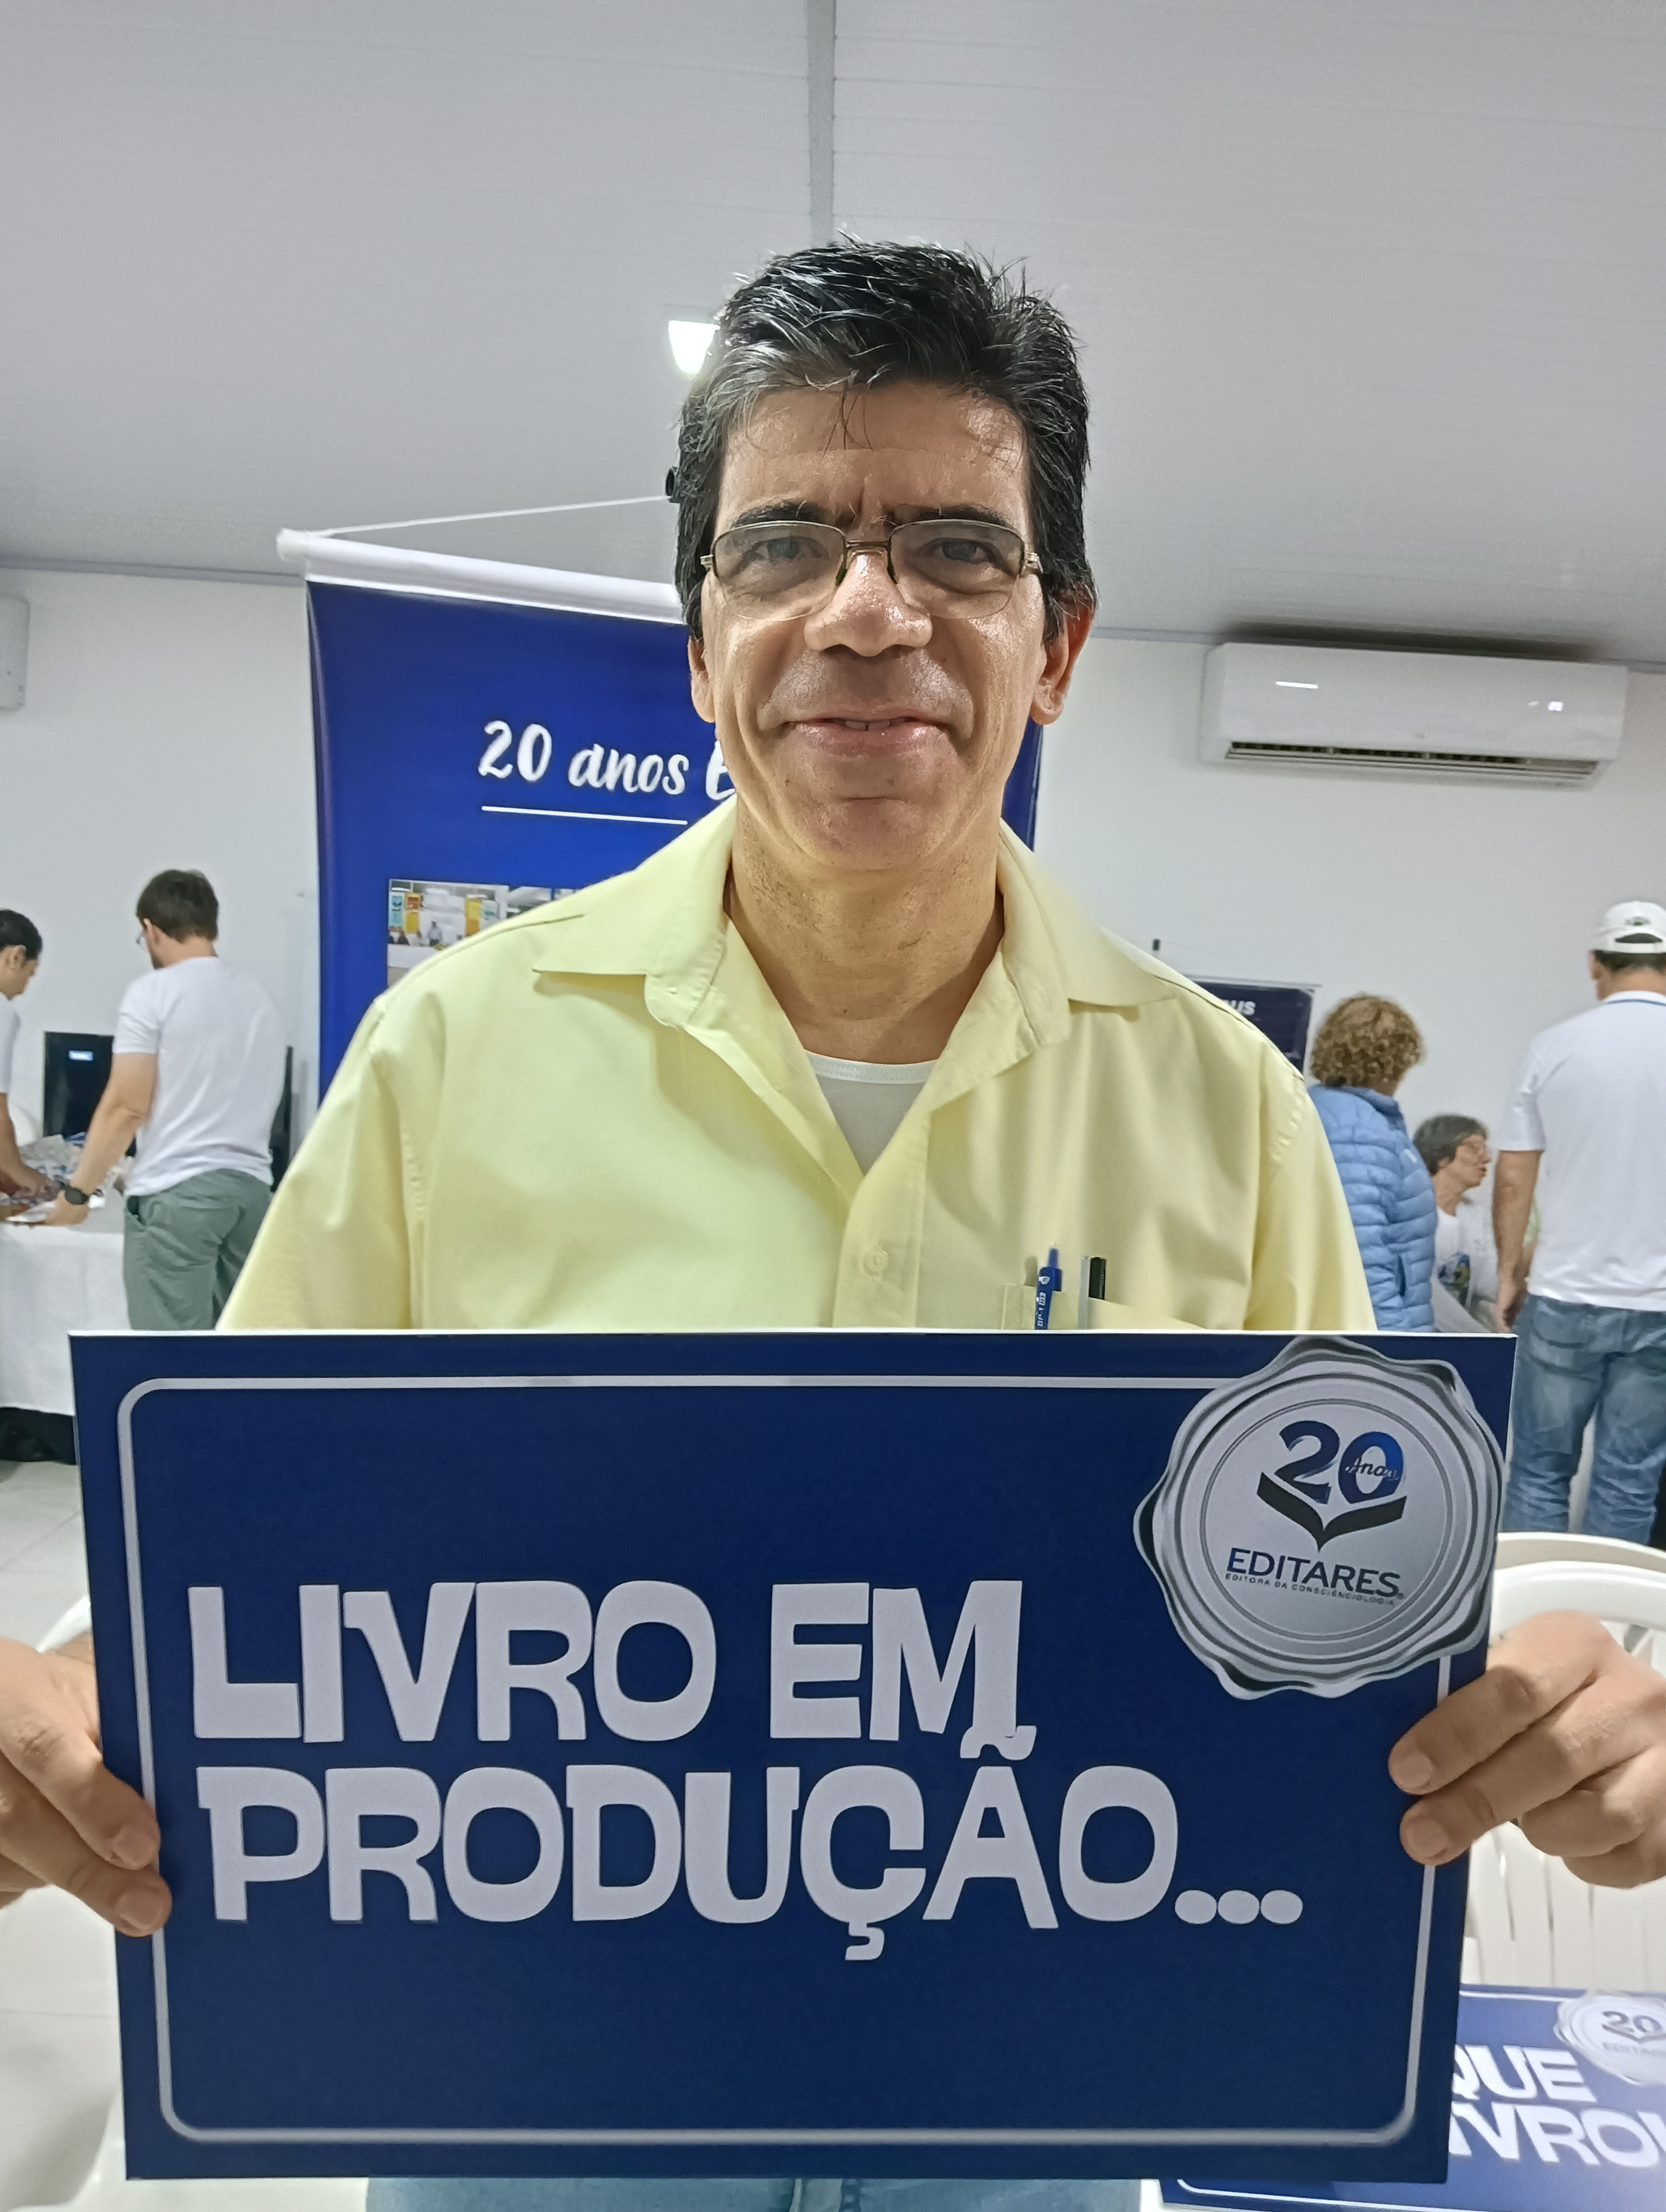
\includegraphics[height=5cm]{articles/resumo/fotos/materia2/IMG20241208144653.jpg}
  \end{minipage}\hfill
  \begin{minipage}[b]{0.55\textwidth}
    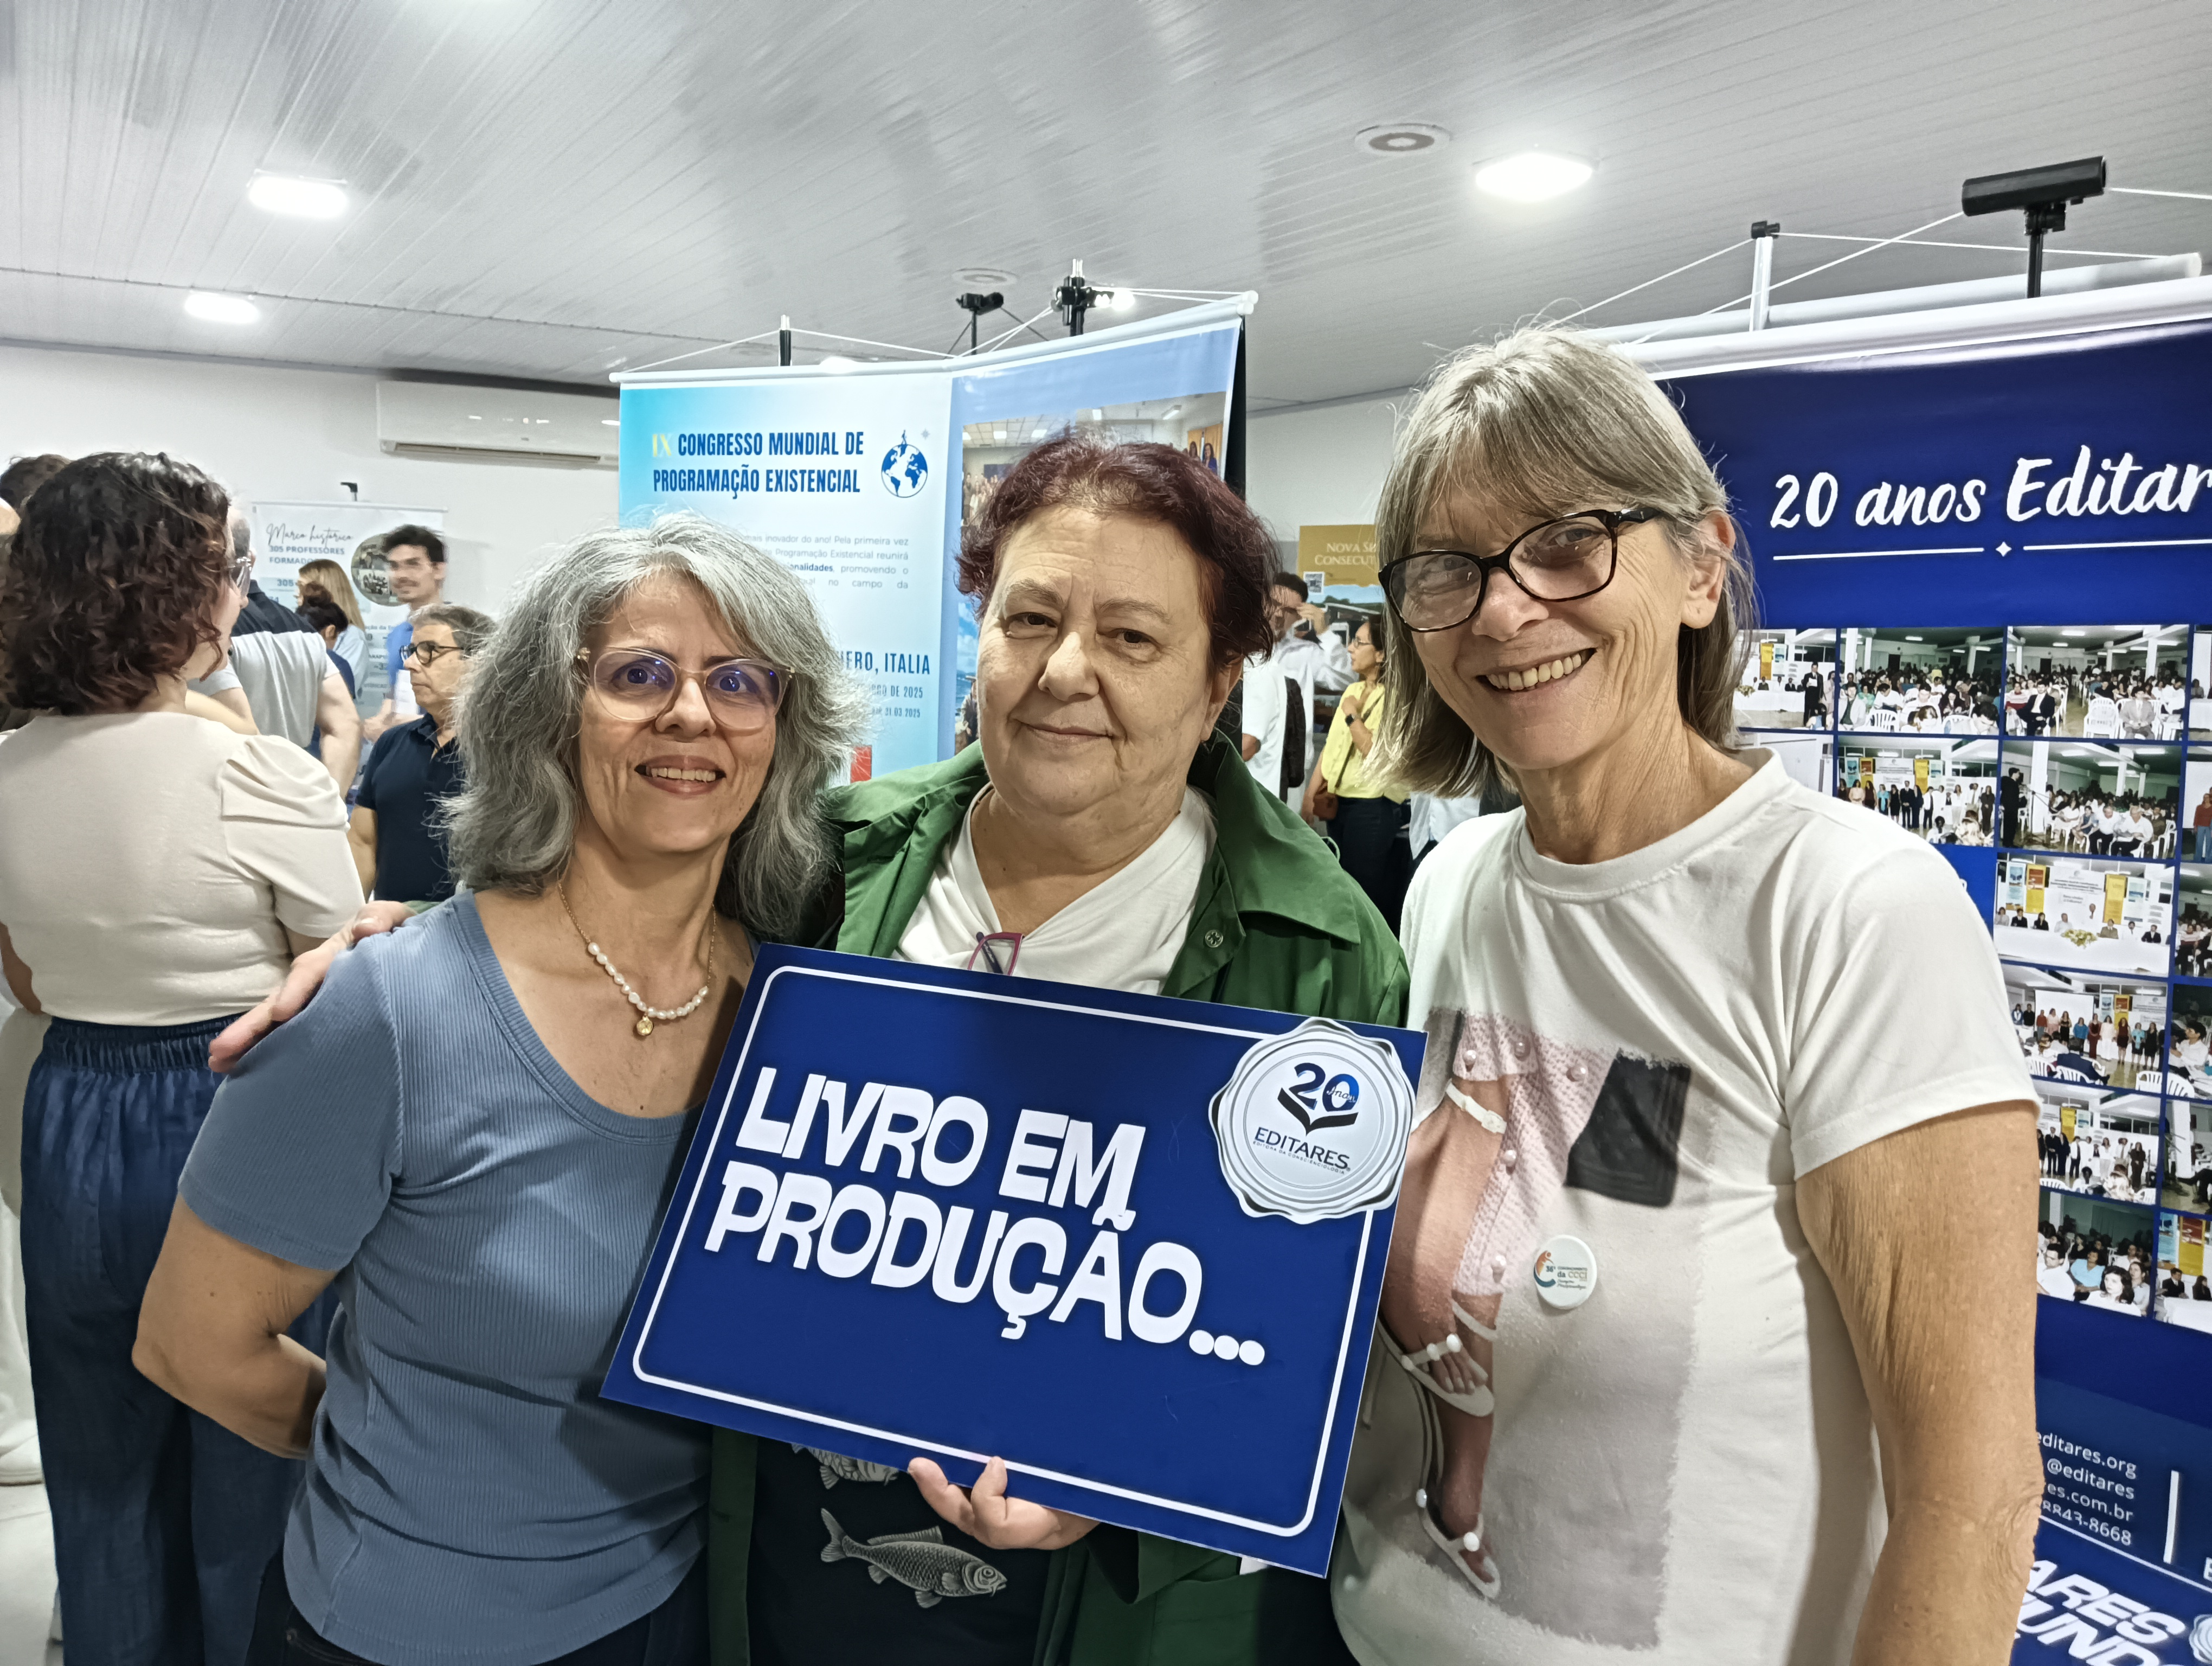
\includegraphics[height=5cm]{articles/resumo/fotos/materia2/IMG20241208155101.jpg}
  \end{minipage}

\coverart{../fundo-generico.png}

%{[}MURAL/MOSAICO DE FOTOS{]} Fotos na pasta matéria 2\ldots{} as fotos podem ocupar 2 páginas



        
%    \end{multicols}
\end{document}
